% Self-contained IEEE report: inline bibliography, inline PGFPlots data, and TikZ diagrams.
% Compile twice with pdfLaTeX; no BibTeX, external images, CSV files, or shell escape needed.
% Requires standard installed packages IEEEtran, pgfplots and TikZ (provided by Overleaf).
\documentclass[conference]{IEEEtran}
\usepackage{amsmath,amssymb,bm,booktabs,graphicx,tabularx,array}
\usepackage{tikz,pgfplots,pgfplotstable}
\pgfplotsset{compat=1.18}
\usepgfplotslibrary{groupplots}
\pgfplotsset{reportaxis/.style={width=0.94\columnwidth,height=0.67\columnwidth,
  label style={font=\fontsize{9}{11}\selectfont},
  tick label style={font=\fontsize{9}{10}\selectfont},
  legend style={font=\fontsize{9}{10}\selectfont,draw=none,fill=white},
  grid=major,grid style={black!12},mark size=1.3pt,clip=true}}
\usetikzlibrary{arrows.meta,positioning}
\usepackage[hidelinks]{hyperref}
\newcolumntype{Y}{>{\raggedright\arraybackslash}X}
\newcommand{\E}{\mathbb{E}}
\newcommand{\F}{\mathbf{F}}
\newcommand{\J}{\mathbf{J}}
\title{Identifiability-Guided Active Calibration for Semi-Supervised ISAC:\\Baseline Reproduction and Extended Evaluation}
\author{\IEEEauthorblockN{Muneef Mohammed, Andrew Liang, and Mohammad Al-Shammeri}
\IEEEauthorblockA{CISC 867: Deep Learning, Queen's University\\Updated midterm report: experiments through November 8, 2026}\\
\textbf{GitHub Repository:} \url{https://github.com/andrewliang-uwcs/867-deep-learning}}
\pgfplotstableread{
x y
1.0000000000 0.17507789080
200.00000000 0.15504450710
400.00000000 0.14268434369
600.00000000 0.13500948631
700.00000000 0.13248621262
800.00000000 0.12971113825
1000.0000000 0.12526719288
1500.0000000 0.11073759550
2000.0000000 0.095768142221
2500.0000000 0.088214919857
3000.0000000 0.083922440324
3500.0000000 0.079962233666
5000.0000000 0.071361218199
6500.0000000 0.069867067691
8000.0000000 0.067264737950
10000.000000 0.064530990492
}\MeasuredSL
\pgfplotstableread{
x y
1.0000000000 6.3385435869
200.00000000 4.4637768709
400.00000000 3.9751347415
600.00000000 3.6163486416
700.00000000 3.4324377805
800.00000000 3.5075648916
1000.0000000 3.4251652301
1500.0000000 3.2136033350
2000.0000000 2.8417235154
2500.0000000 2.6845968697
3000.0000000 2.5910281541
3500.0000000 2.5056671162
5000.0000000 2.5142228747
6500.0000000 2.6963097484
8000.0000000 2.3051556319
10000.000000 2.4727785845
}\LocalizationSL
\pgfplotstableread{
x y
1.0000000000 0.17407412099
200.00000000 0.11464578129
400.00000000 0.10151205178
600.00000000 0.098562230941
700.00000000 0.097685180771
800.00000000 0.097635256739
1000.0000000 0.097273540598
1500.0000000 0.096235727474
2000.0000000 0.097212915540
2500.0000000 0.097087611592
3000.0000000 0.096904207599
3500.0000000 0.096394516723
5000.0000000 0.096611938174
6500.0000000 0.097370369431
8000.0000000 0.096747907310
10000.000000 0.096671070705
}\MeasuredUL
\pgfplotstableread{
x y
1.0000000000 6.3992178674
200.00000000 3.3931195552
400.00000000 3.1809534175
600.00000000 3.1345822429
700.00000000 3.2499497820
800.00000000 3.1366535778
1000.0000000 3.1839184453
1500.0000000 3.2561678008
2000.0000000 3.2652108481
2500.0000000 3.1864110682
3000.0000000 3.1233621984
3500.0000000 3.2399125217
5000.0000000 3.0590971539
6500.0000000 3.2684649556
8000.0000000 3.1091751237
10000.000000 3.2709583416
}\LocalizationUL
\pgfplotstableread{
x y
100.00000000 0.17494529328
85000.000000 0.17494529328
}\BaselineDetection
\pgfplotstableread{
x y
100.00000000 6.4303271028
85000.000000 6.4303271028
}\BaselineLocalization
\pgfplotstableread{
x y
0.99999995831 0.17425832177
199.98159649 0.15607121472
399.99958368 0.14513581557
599.98536458 0.13995427452
699.92539460 0.13707166381
799.99911788 0.13438161727
999.99983325 0.12949572684
1499.9654728 0.11329846085
1999.8164651 0.099613544814
2499.9642509 0.086316989195
2999.9262581 0.081208084973
3499.6280648 0.078100180997
4999.9256914 0.070535165074
6499.5728958 0.068427403990
7999.9891778 0.067864681146
10000.000834 0.066211963474
12499.831407 0.064823732343
14999.650977 0.063498986146
19998.159649 0.062570561498
24999.623750 0.059171361694
29999.285091 0.058953349120
34996.254388 0.058393314009
39999.938359 0.059351609918
44999.227432 0.058730029123
49999.244408 0.056831128712
54998.104821 0.056280585722
59998.506445 0.057277666639
64995.777728 0.056697150323
69992.504447 0.056342097384
74986.836533 0.056502000490
79999.871769 0.056926492202
84997.134142 0.055847724613
}\PaperSL
\pgfplotstableread{
x y
0.99999995831 0.17486551128
199.98159649 0.14369488446
399.99958368 0.12243777388
599.98536458 0.11080421055
699.92539460 0.10644535396
799.99911788 0.10464783893
999.99983325 0.10116514929
1499.9654728 0.10000993441
1999.8164651 0.096582258240
2499.9642509 0.096840518767
2999.9262581 0.096601922920
3499.6280648 0.095957241229
4999.9256914 0.098163767998
6499.5728958 0.097742236194
7999.9891778 0.096797310906
10000.000834 0.097182915544
12499.831407 0.098436691979
14999.650977 0.098213644158
19998.159649 0.098226198253
24999.623750 0.097065982145
29999.285091 0.098290329605
34996.254388 0.098004137068
39999.938359 0.095904371139
44999.227432 0.095698096132
49999.244408 0.095342873085
54998.104821 0.095946898560
59998.506445 0.095255776925
64995.777728 0.097985561090
69992.504447 0.094717822052
74986.836533 0.095946082034
79999.871769 0.096097479655
84997.134142 0.094739664135
}\PaperUL
\pgfplotstableread{
x y
0.0076863900758 0.99009811387
0.0077086621895 0.98995782337
0.0077242054977 0.98954745315
0.0077396128327 0.61954003726
0.0084185739979 0.42205103217
0.0095474673435 0.32247048552
0.011384456418 0.26575644828
0.011439833790 0.26415341991
0.014712984674 0.22454690783
0.022927077487 0.19505557355
0.53176903725 0.17473538653
0.53189104795 0.17425753661
0.53197187185 0.17401886337
}\BaselineJointDetection
\pgfplotstableread{
x y
0.0076863900758 83.641956194
0.0077098337933 82.888986113
0.0077127311379 81.200685330
0.0077396128327 12.105791492
0.0084185739979 9.0644957851
0.0090239224955 8.7893919561
0.0095474673435 7.8961670363
0.0096956156194 7.7095016331
0.011384456418 7.3607649318
0.011439833790 7.3397387348
0.012285390869 7.2794242102
0.012699984014 7.2656033054
0.014452301897 7.1511913905
0.014712984674 6.7246179935
0.015981797129 6.6276494473
0.022927077487 6.3053346256
0.53176903725 6.2905616580
}\BaselineJointLocalization
\pgfplotstableread{
x y
0.0013143327087 0.98845056373
0.0013167252764 0.98844335673
0.0013274055673 0.98835190163
0.0015008789487 0.35644595396
0.0015218944754 0.34892585823
0.0015454362147 0.34739939162
0.0017941829283 0.20175194343
0.0018172070850 0.19891191024
0.0018440950662 0.19796544737
0.0022284765728 0.14159251388
0.0022394564003 0.14029318434
0.0022749870550 0.13812808431
0.0029564616270 0.10921852200
0.0029573601205 0.10736917145
0.0030087435152 0.10687960359
0.0044180955738 0.088205947049
0.0044213901274 0.087319909322
0.0045514386147 0.086945174678
0.0085955439135 0.074825785238
0.0086771482602 0.073637638528
0.36525952816 0.064800366918
0.36557662487 0.064672812987
0.36565452814 0.064542958998
0.36567062140 0.064164922374
0.36570385098 0.063975410551
}\SLJointDetection
\pgfplotstableread{
x y
0.0013143327087 77.168218736
0.0013173340121 76.074270626
0.0015008789487 6.4373557124
0.0015166015364 6.2529963293
0.0015218944754 6.1886138686
0.0015454362147 6.1081438051
0.0017941829283 4.3422460602
0.0018440950662 4.3188970877
0.0022284765728 3.5874655862
0.0022749870550 3.5124624496
0.0023489224259 3.4183258650
0.0029564616270 3.0704935551
0.0031101789791 3.0337257414
0.0044180955738 2.8376077361
0.0044213901274 2.8079354987
0.0044984114356 2.7650552573
0.0047349054366 2.7526694432
0.0047718910500 2.7492943588
0.0085955439135 2.4317064875
0.0091615822166 2.4143979924
0.36525952816 2.3645288402
0.36527442932 2.1765351552
}\SLJointLocalization
\pgfplotstableread{
x y
0.0012548242230 0.98946321022
0.0012571223779 0.98929936604
0.0014527473832 0.45708966247
0.0017409733264 0.28061536177
0.0021515430417 0.20275383472
0.0028301042039 0.15888418649
0.0041575455107 0.13109206730
0.0045411358587 0.13085518019
0.0080053219572 0.11077824836
0.29254966974 0.096647582471
}\ULJointDetection
\pgfplotstableread{
x y
0.0012548242230 80.238591966
0.0012558919843 79.875058004
0.0014527473832 8.1941923079
0.0014566276222 8.1610573443
0.0014670150122 7.9575359062
0.0017409733264 5.5322222650
0.0017534537474 5.4547103656
0.0021515430417 4.5947975846
0.0022339355201 4.5397470626
0.0028301042039 4.0595625444
0.0028756249230 3.9689244695
0.0029169823974 3.8493412485
0.0041575455107 3.7429198121
0.0043419334106 3.7002950512
0.0045213899575 3.6011858216
0.0045411358587 3.5694556757
0.0080053219572 3.2902795725
0.29254966974 3.2602963456
0.29267945886 3.1772317663
0.29286962748 3.1597989543
}\ULJointLocalization
\pgfplotstableread{
x y
0.0077368430587 0.98972412985
0.0077126764752 0.61816934388
0.0083559490523 0.42151862412
0.0095599969476 0.32259086642
0.011310930778 0.26373847176
0.014663143484 0.22452920241
0.023139236071 0.19506362712
0.53205247498 0.17410014200
}\PaperJointBaselineDetection
\pgfplotstableread{
x y
0.0012452990745 0.98840378379
0.0014416223812 0.30520292178
0.0017005140047 0.17367242642
0.0021198463596 0.12286602544
0.0027733378225 0.094218621893
0.0040520892756 0.077512846202
0.0077469985826 0.065027237607
0.38138556431 0.055787472512
}\PaperJointSLDetection
\pgfplotstableread{
x y
0.0077368430587 84.748235413
0.0077126764752 12.119433424
0.0083559490523 9.0398419543
0.0095599969476 7.8850279263
0.011310930778 6.9728769753
0.014663143484 6.9667522593
0.023139236071 6.4855689556
0.53205247498 6.4006765503
}\PaperJointBaselineLocalization
\pgfplotstableread{
x y
0.0012452990745 78.001732349
0.0014416223812 5.7565005460
0.0017005140047 3.9604247666
0.0021198463596 3.2583139359
0.0027733378225 2.6454958590
0.0040520892756 2.6115093698
0.0077469985826 2.4065731823
0.38138556431 2.1281011329
}\PaperJointSLLocalization

\pgfplotstableread{
x y err
10.00000000 0.3122448327 0.1025309974
15.00000000 0.2104635412 0.07617585500
20.00000000 0.1894636753 0.05930301002
25.00000000 0.1722859506 0.04189098907
30.00000000 0.1653193889 0.04389479078
35.00000000 0.1641369275 0.04012756697
40.00000000 0.1558305815 0.03191420292
45.00000000 0.1632943854 0.02762481615
50.00000000 0.1600610840 0.02234842916
55.00000000 0.1613780592 0.05616589450
60.00000000 0.1615954511 0.03719130286
}\Activeweak
\pgfplotstableread{
x y err
10.00000000 0.3127896877 0.1026792621
15.00000000 0.2123017356 0.07634208879
20.00000000 0.1825003914 0.06524937056
25.00000000 0.1735140467 0.04158791046
30.00000000 0.1656300271 0.04359893077
35.00000000 0.1635055140 0.03984801670
40.00000000 0.1556203562 0.03336547865
45.00000000 0.1651286368 0.02575233674
50.00000000 0.1582952471 0.01607672681
55.00000000 0.1594681790 0.04994512709
60.00000000 0.1555401861 0.02765027249
}\Activefull
\pgfplotstableread{
x y err
10.00000000 0.3127896877 0.1026792621
15.00000000 0.2132187011 0.07696721459
20.00000000 0.1843886210 0.07421795809
25.00000000 0.1962861222 0.06237323264
30.00000000 0.1953549053 0.05740854997
35.00000000 0.1937010196 0.05007012660
40.00000000 0.1879424410 0.04037968847
45.00000000 0.1944199244 0.03539616546
50.00000000 0.1906413914 0.03163933533
55.00000000 0.1886519180 0.04666919985
60.00000000 0.1977882045 0.03927101211
}\Activerandom
\pgfplotstableread{
x y
10.00000000 0.3127896877
15.00000000 0.2225
20.00000000 0.1951
25.00000000 0.1922
30.00000000 0.2059
35.00000000 0.2169
40.00000000 0.2059
45.00000000 0.2082
50.00000000 0.2070
55.00000000 0.2023
60.00000000 0.1947
}\Activemaxangle
\pgfplotstableread{
x y
10.00000000 0.3127896877
15.00000000 0.2208
20.00000000 0.2093
25.00000000 0.2010
30.00000000 0.1971
35.00000000 0.1950
40.00000000 0.1904
45.00000000 0.1890
50.00000000 0.1825
55.00000000 0.1871
60.00000000 0.1836
}\Activediversity
\pgfplotstableread{
x y
10.00000000 0.3127896877
15.00000000 0.2207
20.00000000 0.2080
25.00000000 0.2269
30.00000000 0.2472
35.00000000 0.2644
40.00000000 0.2852
45.00000000 0.3071
50.00000000 0.3133
55.00000000 0.3231
60.00000000 0.3305
}\Activeuncertainty
\pgfplotstableread{
x y
1 0.17507789
200 0.15504451
400 0.14268434
600 0.13500949
700 0.13248621
800 0.12971114
1000 0.12526719
1500 0.06906698
2000 0.05856147
2500 0.05888377
3000 0.05861301
3500 0.05853806
5000 0.05893117
6500 0.0578652
8000 0.05884106
10000 0.0584767761809
}\MeasuredSSL
\pgfplotstableread{
x y
1 6.33854359
200 4.46377687
400 3.97513474
600 3.61634864
700 3.43243778
800 3.50756489
1000 3.42516523
1500 2.62146822
2000 2.18627647
2500 2.21369283
3000 2.25104616
3500 2.2982563
5000 2.27709382
6500 2.08501045
8000 2.07218304
10000 2.1587240158
}\LocalizationSSL

\pgfplotstableread{
x y
1.0000684585 0.17425831784
199.96003182 0.1560712289
400.03046934 0.14513580866
599.98652481 0.13995426172
699.8950631 0.13707166692
799.90273398 0.13438163469
1000.0630346 0.12949572137
1499.9708332 0.10215977724
1999.6099811 0.095853186304
2500.1651226 0.089810765978
2999.9427786 0.086308130853
3499.5361484 0.082915504978
5000.2513341 0.074214348471
6499.4171004 0.068925816148
7999.0573812 0.062191840209
10000.818668 0.057659125226
12500.854466 0.057516243061
14999.732362 0.05863618545
19996.196441 0.058979718548
25001.745122 0.059177549683
29999.508149 0.058004476352
34994.965354 0.058725714056
40003.390483 0.059489248739
45001.753135 0.058875163383
50002.701132 0.057824751292
55001.165827 0.059572803825
59999.103147 0.058271466759
64994.415098 0.058843143828
69990.032019 0.058885329499
74980.585672 0.058326972269
80006.724474 0.059119484093
85000.484617 0.058836576665
}\PaperSSL
\pgfplotstableread{
x y
0.0012318691475 0.98967371399
0.001233486788 0.98958311781
0.0012340899814 0.98955304942
0.0012452689996 0.98926590382
0.0014232517774 0.31285859308
0.0016917059997 0.17997261245
0.002097895857 0.12791220026
0.0021166740186 0.12768985759
0.0027602521553 0.098355437027
0.0027900208282 0.098156018597
0.0040560718606 0.080622828567
0.0040906930678 0.079628878524
0.0077237302224 0.067771196723
0.0079146200834 0.067668892208
0.4841089444 0.058685121366
0.48426378899 0.058424217359
}\SSLJointDetection
\pgfplotstableread{
x y
0.001231862753 82.248237528
0.0012334803831 81.857596079
0.0012340835726 80.150683019
0.0014232441282 5.8263588416
0.0016916965362 4.1848201657
0.001724481986 4.1671053764
0.0017358088231 4.1131550966
0.0020978835474 3.372335654
0.0021166615748 3.2459124463
0.0022096964042 3.2152011162
0.0027602349965 2.9443090699
0.0027900034462 2.8983950131
0.0029491726093 2.8492375124
0.0029603087189 2.7945112847
0.0040560446619 2.57689226
0.007723672106 2.3497561744
0.48410275535 2.0792522814
}\SSLJointLocalization
\pgfplotstableread{
x y
0.0012390145134 0.98953801557
0.0014291065917 0.31330302432
0.0016860107104 0.18009352166
0.0021010028719 0.12726576381
0.0027510859099 0.098129103256
0.0040324997493 0.0807545947
0.0077432030399 0.067486405511
0.49233329151 0.058643071943
}\PaperSSLJointDetection
\pgfplotstableread{
x y
0.0012390080727 83.120060657
0.0014290989036 5.9353858619
0.001686001286 4.0799617957
0.00210099054 3.4927942663
0.0027510688197 2.7223276182
0.0040324727386 2.655613495
0.0077431447522 2.4020694327
0.49232698676 2.1390786957
}\PaperSSLJointLocalization

\pgfplotstableread{
x y
1 0.174329256552
200 0.158581451077
400 0.145245583811
600 0.138297629163
700 0.13610897302
800 0.133825393261
1000 0.12766464152
1500 0.115747228377
2000 0.104262963238
2500 0.0945734202309
3000 0.0867619178393
3500 0.0830976103947
5000 0.0739329838085
6500 0.0725167407609
8000 0.0717144274692
10000 0.0672030589529
12500 0.0652658611612
15000 0.0667651884562
20000 0.0602536363229
25000 0.0605066026674
30000 0.0615328765056
35000 0.0623472354463
40000 0.0635645537827
45000 0.061192689112
50000 0.0589194611366
55000 0.0591717653389
60000 0.0589788004701
65000 0.0581651819353
70000 0.0581484650836
75000 0.0583948237871
80000 0.0583260198726
81000 0.0583648329599
82000 0.0580645374989
83000 0.0576381756214
84000 0.0580441160123
84200 0.0577756646832
85000 0.0578086942427
}\FullDetectionSL
\pgfplotstableread{
x y
1 6.4301906263
200 4.41911639119
400 4.04939431868
600 3.87356279386
700 3.77274248778
800 3.57168067424
1000 3.31557635668
1500 3.14058715076
2000 3.12330490989
2500 2.83904107901
3000 2.83098806539
3500 2.54883480387
5000 2.66205721589
6500 2.4037617926
8000 2.43703209577
10000 2.29800762752
12500 2.2935429837
15000 2.52957618963
20000 2.29782778346
25000 2.16878521722
30000 2.297558163
35000 2.19729083929
40000 2.17621482147
45000 2.27363077388
50000 2.28520713026
55000 2.09578784267
60000 2.21607288667
65000 2.07337947182
70000 2.20534498122
75000 2.31355110715
80000 2.15597466912
81000 2.12792440268
82000 2.1446030932
83000 2.19747722381
84000 2.12369269092
84200 2.14214082958
85000 2.29433858324
}\FullLocalizationSL
\pgfplotstableread{
x y
1 0.173759174751
200 0.113501461334
400 0.101611380613
600 0.0987292686791
700 0.0976770348867
800 0.0971167609843
1000 0.0970451744589
1500 0.0969571786693
2000 0.096556433669
2500 0.0972129324886
3000 0.0966802109337
3500 0.0965849996486
5000 0.0971790212516
6500 0.0965283264385
8000 0.096868659792
10000 0.0960677561293
12500 0.0972357682114
15000 0.0968549032959
20000 0.097516289622
25000 0.0969778236162
30000 0.0967985808588
35000 0.0974008058306
40000 0.0983298567684
45000 0.0975486696315
50000 0.0968680747072
55000 0.0960507486322
60000 0.0970477193677
65000 0.0968469850132
70000 0.0969108172099
75000 0.0964624492593
80000 0.0963478741901
81000 0.0965805623295
82000 0.0967844816505
83000 0.0963623378645
84000 0.096464232194
84200 0.0971817536613
85000 0.0973715761076
}\FullDetectionUL
\pgfplotstableread{
x y
1 6.42512216081
200 3.46776674492
400 3.45962922798
600 3.24561421665
700 3.08663691058
800 3.46175731761
1000 3.1770870192
1500 3.17595758139
2000 3.2946073657
2500 3.17047868407
3000 3.14678423931
3500 3.22801110097
5000 3.14809965493
6500 3.23951769255
8000 3.16614912135
10000 3.24328439127
12500 3.12715709053
15000 3.27147007541
20000 3.28020031061
25000 3.09356200785
30000 3.25231257552
35000 3.33162395283
40000 3.35404866656
45000 3.21613170558
50000 3.15017438614
55000 3.34004681449
60000 3.18913891035
65000 3.12799584972
70000 3.27126824345
75000 3.25723264945
80000 3.19611665646
81000 3.30706793616
82000 3.1098845603
83000 3.27101417758
84000 3.25582814557
84200 3.22056238181
85000 3.30526530244
}\FullLocalizationUL
\pgfplotstableread{
x y
1 0.175077890802
200 0.155044507104
400 0.142684343689
600 0.135009486315
700 0.13248621262
800 0.129711138247
1000 0.125267192881
1500 0.0690669799103
2000 0.0585614670576
2500 0.0588837696518
3000 0.0586130111555
3500 0.0585380629017
5000 0.0589311702132
6500 0.0578652005548
8000 0.0588410589641
10000 0.0584767761809
12500 0.0588568660083
15000 0.0582811036751
20000 0.059004453198
25000 0.0584155984607
30000 0.0586944132969
35000 0.0585667034442
40000 0.058501171914
45000 0.0584784167223
50000 0.0584102104679
55000 0.0583188252577
60000 0.0585024742574
65000 0.0581213642645
70000 0.0586724896612
75000 0.0583796987649
80000 0.0585204719543
81000 0.0590697173901
82000 0.0588545243157
83000 0.0583048615943
84000 0.0588669360739
84200 0.0585508704939
85000 0.0584079892678
}\FullDetectionSSL
\pgfplotstableread{
x y
1 6.33854358694
200 4.46377687085
400 3.97513474153
600 3.61634864159
700 3.43243778054
800 3.50756489161
1000 3.42516523008
1500 2.62146822211
2000 2.18627647288
2500 2.21369282866
3000 2.25104615683
3500 2.29825629724
5000 2.27709382339
6500 2.08501045128
8000 2.07218303758
10000 2.1587240158
12500 2.32066267819
15000 2.27058988109
20000 2.20486917208
25000 2.23501119853
30000 2.11539106011
35000 2.23212158327
40000 2.07417866519
45000 2.1883244093
50000 2.46194899334
55000 2.17054065877
60000 2.17115173878
65000 2.21818763434
70000 2.16101221472
75000 2.15900647811
80000 2.26964557742
81000 2.22072532774
82000 2.40795481749
83000 2.30574767437
84000 2.18310292137
84200 2.18987477119
85000 2.18035482067
}\FullLocalizationSSL

\begin{document}
\maketitle
\begin{abstract}
We study identifiability-guided position-label acquisition for semi-supervised integrated sensing and communication (ISAC). Extending our midterm reproduction, we complete supervised (SL), unsupervised (UL), and sequential semi-supervised (SSL) training at 85,000 updates. SSL uses 1,000 SL and 84,000 UL updates and reaches misdetection probability 0.05841 and conditional position RMSE 2.180 m, compared with 0.05781 and 2.294 m for full SL: similar detection with 98.8\% fewer supervised updates in this single-run comparison. We repair checkpoint aliasing and isolate acquisition randomness, then complete 50 matched active-calibration runs across five optimization seeds, followed by transfer and central-sector detection/SER evaluation. Guided acquisition has lower mean calibration error than random selection, but its paired interval includes zero; central-sector detection is nearly identical. A further 126 training runs span three independent array draws, two angular coverages, three optimization seeds, and seven variants. Weak-direction, full-trace, D-optimal, and noRC variants select identical labels in all 72 comparisons. Reconstructed candidate information gains are nearly proportional, explaining the lack of criterion separation. Fixed-label controls match or improve mean outcomes, and the guided-versus-random intervals include zero. Thus SSL reproduction is supported, while a distinct active-acquisition advantage is not established. Remaining work includes a labeled-fraction sweep, SNR variation, and separately calibrated operating-point evaluation.

\end{abstract}
\begin{IEEEkeywords}
ISAC, model-based learning, semi-supervised learning, active calibration, label acquisition.
\end{IEEEkeywords}

\section{Introduction}
Integrated sensing and communication (ISAC) shares radio signals and hardware between environmental sensing and data delivery. Both tasks depend on accurate array responses. Antenna-location errors distort transmit beams and received-signal models, degrading detection, localization, and communication. Differentiable model-based learning embeds trainable calibration parameters within a physical processing pipeline, enabling structured adaptation without replacing every component with a generic neural network~\cite{icc,multi}.

Mateos-Ramos \emph{et al.}~\cite{ssl} introduce an unsupervised sensing objective for a single-target ISAC system and train it sequentially: supervised learning (SL) on labeled target positions, followed by unsupervised learning (UL) on unlabeled measurements. We refer to this sequence as semi-supervised learning (SSL). In their setting, SSL approaches SL performance with 98.8\% fewer labeled training samples. Acquiring reference positions may still require external sensors or controlled calibration, which raises a complementary question: \emph{which} positions should be labeled?

This project investigates \emph{whether position labels selected to inform weak hardware-calibration directions improve learning relative to random acquisition under matched budgets}. Unknown target geometry and hardware parameters can affect measurements similarly, so unlabeled observations may leave some calibration directions weakly constrained, while selected position references provide complementary information. As in our proposal, we keep the hardware fixed and consider a single target. Local information analysis guides the design; it does not establish global identifiability.

This midterm report makes three contributions:
\begin{enumerate}
\item A completed 85,000-update SL/UL/SSL comparison in addition to the original 10,000-update reproduction.
\item Repaired acquisition experiments with fixed-label, full-trace and noRC controls, and detection/SER evaluation across five optimization seeds.
\item A 126-run robustness study over independent hardware draws and angular coverage, and diagnostics explaining identical information-based selections. These experiments do not establish a unique benefit from weak-direction targeting.


\end{enumerate}

\section{Related Work}
\emph{Model-based learning and ISAC calibration.} Model-based deep learning combines domain-specific signal models with trainable components. Shlezinger \emph{et al.}~\cite{mbdl} review strategies that incorporate mathematical structure into learning systems, including communication and estimation applications. This perspective motivates our differentiable calibration parameters and structured receiver, but does not determine which observations should receive supervision.

Mateos-Ramos \emph{et al.}~\cite{icc} embed trainable steering matrices in a model-driven ISAC transceiver with $K=16$ antennas and compare it with a neural network under antenna-spacing errors of standard deviation $\lambda/30$. Without complexity limits, the network (about 6.4 million real parameters) slightly outperforms the model-driven design (8,000 complex parameters). When both are restricted to a few thousand parameters (about 5,000 real versus 2,500 complex), the network degrades while the model-driven design stays close to its unrestricted performance and generalizes better to an unseen angular sector. The semi-supervised framework~\cite{ssl} that we reproduce uses $K=64$ antennas, an unsupervised loss that maximizes the peak of the angle--delay map, and SL followed by UL. Over 85,000 total updates, spending about 1.2\% of them on SL matches full SL, whereas performance degrades when the labeled fraction falls below about 1\%. We reproduce this framework and study how reference positions are chosen, distinguishing unique acquired labels from their repeated use during optimization.

Several studies extend impairment learning. The multi-target framework~\cite{multi} uses a differentiable orthogonal matching pursuit for up to five targets with $K=64$. Learning the 64 spacing parameters directly, rather than a $64\times720$ dictionary (46,080 complex parameters), approaches the detection performance of a baseline with known impairments at $P_{\rm fa}=10^{-2}$ and converges faster. Gain--phase calibration~\cite{gain} learns per-antenna complex gain errors of a 64-element array without labels ($10^4$ updates, batch 1,024), with sensing performance close to the known-impairment case. Physically parameterized differentiable MUSIC (multiple signal classification)~\cite{music} learns antenna-location and complex-gain errors with supervised or unsupervised losses and estimates direction of arrival more accurately than classical MUSIC. A later multi-target preprint~\cite{multiul} calibrates arrays without labels using coherent received signals and alternative sensing objectives. All of these methods learn from unlabeled or randomly labeled data; none decides which observations to label.

\emph{Calibration ambiguity and statistical acquisition.} Weiss and Friedlander~\cite{weiss} estimate sensor locations jointly with the directions of sources at unknown locations by maximum likelihood. Their formulation exposes the coupling between hardware and target parameters that our nuisance elimination accounts for, and global motions of the array that such data cannot observe---the analogue of the translation gauge we remove in~\eqref{eq:calib}. Cohn, Ghahramani, and Jordan~\cite{cohn} derive closed-form query criteria that minimize the expected variance of a learner (mixtures of Gaussians and locally weighted regression) rather than maximizing prediction uncertainty. Our calibration-specific hypothesis follows the same logic: some uncertain positions carry less information about shared hardware than observations sensitive to its weak directions.

\emph{Diversity, gradient, and information-based selection.} Core-set acquisition~\cite{coreset} casts batch selection as a $k$-center problem in a network's feature space and reports gains over random and uncertainty sampling on image classification benchmarks (CIFAR-10/100, Caltech-256, SVHN). Our estimated-angle diversity rule is a simpler, task-specific version. BADGE~\cite{badge} samples diverse, high-magnitude last-layer gradient embeddings by $k$-means++ seeding; transferring it to position regression would require replacing its hallucinated class labels. BAIT~\cite{bait} greedily minimizes $\operatorname{tr}((\sum_{x\in S}\mathbf I(x))^{-1}\mathbf I_U)$, a trace criterion on last-layer Fisher information, oversampling $2B$ candidates and pruning to $B$. It matches or outperforms BADGE, Core-set, confidence, and random sampling on MNIST, SVHN, CIFAR-10, and OpenML classification and on regression tasks; its authors prefer the trace to the log-determinant, which our D-optimal comparator uses. Information-based selection is therefore not our contribution. We study the incremental information a position label provides about shared calibration parameters after nuisance elimination, with emphasis on weak directions that labels can constrain.

Table~\ref{tab:related} summarizes the reviewed works. A fair evaluation requires random, diversity, uncertainty, and conventional information comparators, isolated tests of weak-direction targeting and batch updating, and sensing--communication performance at matched labeling and computational budgets.

\begin{table*}[t]\centering\small
\caption{The 12 reviewed works. Settings and results are as reported by their authors.}\label{tab:related}
\begin{tabularx}{\textwidth}{>{\raggedright\arraybackslash}p{3.2cm}YYp{3.1cm}}\toprule
Work & Setting & Reported result & Role in our study\\\midrule
Model-based DL~\cite{mbdl} & Review of structured learning & Taxonomy of model-based designs & Learning framework\\
Model-driven ISAC~\cite{icc} & $K=16$, one target, spacing errors ($\sigma=\lambda/30$) & 2,500 complex parameters stay near full-complexity performance; a 5,000-parameter network degrades & Preceding architecture\\
Semi-supervised ISAC~\cite{ssl} & $K=64$, $S=256$, 85,000 updates & About 1.2\% supervised updates match full SL; degrades below about 1\% & Reproduction baseline\\
Multi-target ISAC~\cite{multi} & $K=64$, up to 5 targets, 15,000 updates & 64 learned spacings approach known-impairment detection with $720\times$ fewer parameters than a dictionary & Calibration scope\\
Gain--phase calibration~\cite{gain} & $K=64$, unsupervised, $10^4$ updates & Close to known-impairment sensing & Calibration scope\\
Differentiable MUSIC~\cite{music} & Direction of arrival, location and gain errors & More accurate than classical MUSIC & Calibration scope\\
Unsupervised multi-target~\cite{multiul} & Coherent signals, no labels & Preprint; alternative sensing objectives & Subsequent work\\
Array self-calibration~\cite{weiss} & Maximum likelihood, sources at unknown directions & Joint geometry and direction estimates & Nuisance coupling, gauge\\
Statistical acquisition~\cite{cohn} & Variance reduction for regression & Closed-form query criteria & Selection rationale\\
Core-set / BADGE~\cite{coreset,badge} & Feature-space coverage; gradient embeddings & Gains over random and uncertainty sampling on image benchmarks & Diversity comparator\\
BAIT~\cite{bait} & Last-layer Fisher, trace criterion & Matches or beats BADGE and Core-set on classification and regression & Information comparator\\\bottomrule
\end{tabularx}
\end{table*}

\section{System and Implemented Learning Method}
\subsection{Signal model and trainable component}
The transceiver has $K=64$ antenna elements and $S=256$ orthogonal frequency-division multiplexing (OFDM) subcarriers. With $k_c=k-(K-1)/2$ and wavelength $\lambda=c/f_c$, its steering model is
\begin{equation}
 a_k(\theta;\mathbf d)=\exp[-j(2\pi/\lambda)k_c d_k\sin\theta].
 \label{eq:steer}
\end{equation}
Here $k=0,\ldots,K-1$, $c$ is propagation speed, and $j^2=-1$. Parameters $d_k$ induce element positions $k_cd_k$; they are not adjacent gaps. The true fixed vector is $\mathbf d^\star$, while the estimator learns $\widehat{\mathbf d}$, initialized to $(\lambda/2)\mathbf1$. In our code, $\widehat{\mathbf d}$ is the only parameter of a small module (\texttt{PertNet}). Learning occurs by backpropagation through the structured beamformer and receiver rather than through a multilayer predictor.

For a present target at angle $\theta$, range $R$, delay $\tau=2R/c$, and complex reflection gain $\alpha$,
\begin{equation}
 \mathbf Y=\frac{\alpha}{\sqrt S}\mathbf a(\theta;\mathbf d^\star)
 \mathbf a^T(\theta;\mathbf d^\star)\mathbf f
 [\mathbf x\odot\bm\rho(\tau)]^T+\mathbf W,
 \label{eq:obs}
\end{equation}
where $\rho_s(\tau)=e^{-j2\pi s\Delta_f\tau}$, $\mathbf x$ contains known quadrature phase-shift keying (QPSK) symbols, $\mathbf f$ is a unit-norm beam, $\odot$ is elementwise multiplication, and noise entries are independent $\mathcal{CN}(0,N_0)$. For absent targets, $\mathbf Y=\mathbf W$. The physical array remains fixed while its learned model changes.

Reciprocal filtering removes symbols, yielding $\widetilde{\mathbf Y}$. The receiver forms a sector-masked angle--delay map
\begin{equation}
 M_{uv}=\left|\mathbf a^H(\theta_u;\widehat{\mathbf d})
       \widetilde{\mathbf Y}\bm\rho^*(\tau_v)\right|,
\end{equation}
where $H$ and $*$ denote Hermitian transpose and conjugation. The maximum of $M$ selects a window; softmax weighting inside it gives differentiable angle and range estimates and the Cartesian position $\widehat{\mathbf p}=[\widehat R\cos\widehat\theta,\widehat R\sin\widehat\theta]^T$. Note that $\widehat{\mathbf d}$ enters only the angular steering vectors; the delay response $\bm\rho$ does not depend on it.
\begin{figure}[t]\centering
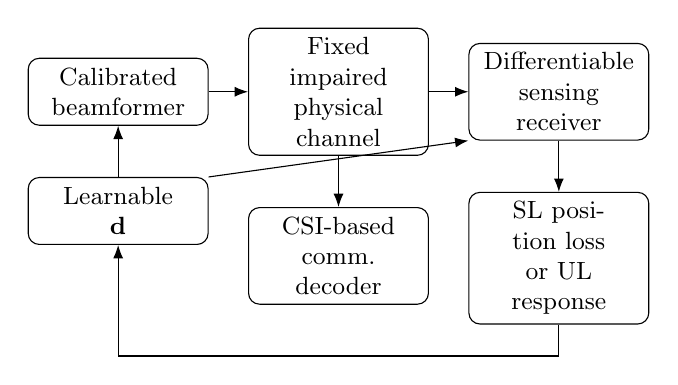
\begin{tikzpicture}[>=Latex,box/.style={draw,rounded corners,align=center,font=\small,text width=2.05cm,minimum height=.85cm},node distance=.5cm]
\node[box] (tx) {Calibrated\\beamformer};
\node[box,right=of tx] (ch) {Fixed impaired\\physical channel};
\node[box,right=of ch] (rx) {Differentiable\\sensing receiver};
\node[box,below=.65cm of tx] (d) {Learnable\\$\mathbf d$};
\node[box,below=.65cm of ch] (comm) {CSI-based\\comm. decoder};
\node[box,below=.65cm of rx] (loss) {SL position loss\\or UL response};
\draw[->] (tx)--(ch);\draw[->] (ch)--(rx);\draw[->] (ch)--(comm);
\draw[->] (rx)--(loss);\draw[->] (d)--(tx);
\draw[->] (d.north east)--(rx.south west);
\draw[->] (loss.south)--++(0,-.4)-|(d.south);
\end{tikzpicture}
\caption{Implemented differentiable pipeline. Gradients update the calibration model while the physical array remains fixed. Scene-label acquisition wraps the supervised and unsupervised updates.}
\label{fig:architecture}
\end{figure}
\subsection{Objectives and communication evaluation}
For minibatch size $B$, the position mean-squared error (MSE) minimized by SL and the peak objective maximized by UL are
\begin{align}
 L_{\rm SL}&=\frac{1}{2B}\sum_i\|\widehat{\mathbf p}_i-\mathbf p_i\|_2^2,\\
 U_{\rm UL}&=\frac1B\sum_i\max_{u,v}M^{(i)}_{uv}.
\end{align}
Both use the Adam optimizer. SL uses present targets. The original online UL randomizes target presence, whereas the pilot uses present-target pools. Labels used for diagnostic metrics never enter the UL objective.

For sensing and communication beams $\mathbf f_r,\mathbf f_c$, joint evaluation sweeps
\begin{equation}
 \mathbf f(\eta,\phi)=
 \frac{\sqrt\eta\mathbf f_r+\sqrt{1-\eta}e^{j\phi}\mathbf f_c}
 {\|\sqrt\eta\mathbf f_r+\sqrt{1-\eta}e^{j\phi}\mathbf f_c\|_2},
\end{equation}
where $\eta\in[0,1]$ controls allocation and $\phi$ is relative phase. The communication receiver uses the effective channel state information (CSI) and maximum-likelihood symbol decisions; imperfect CSI is not studied. The trade-off curves select operating points across beams; they are not a multiobjective training loss.

\subsection{Simulation protocols and metrics}
We use separate configurations for baseline reproduction and the reduced active-calibration pilot (Table~\ref{tab:settings}). The reproduction follows the settings of~\cite{ssl} except for the number of updates; the pilot reduces batch size, training duration, and angular coverage so that repeated comparisons fit on a CPU. Both use a sensing signal-to-noise ratio (SNR) of 15 dB. The completed SSL reproduction uses 1,000 supervised updates followed by 9,000 unsupervised updates, totaling 10,000.

\begin{table}[t]\centering\small
\caption{Reproduction and active-pilot configurations.}\label{tab:settings}
\begin{tabularx}{\columnwidth}{lYY}\toprule
Setting & Reproduction & Active pilot\\\midrule
Antennas / subcarriers & 64 / 256 & Same\\
Carrier / spacing & 60 GHz / 120 kHz & Same\\
Sensing SNR & 15 dB & 15 dB\\
Range / angle grid & 200 / 720 points & Same\\
Range interval & $[0,200]$ m & Same\\
Sector-center support & $[-60,60]^\circ$ & $[-10,10]^\circ$\\
Sector width & $[10,20]^\circ$ & Same\\
Training batch & 3,000 & 64\\
Adam rates, SL/UL & $(4/5)\times10^{-7}$ & $(4/5)\times10^{-6}$\\
Optimizer updates & 10,000 & 2,200\\
Seeds / hardware & One (10) / fixed & Five (0--4) / same fixed\\
Training scenes & Online & 2,000 fixed\\
Evaluation & 1.2M observations & 500 held out\\
Training labels & All for SL & 10 initially; 60 finally\\\bottomrule
\end{tabularx}
\end{table}

Sectors have uniformly sampled centers and widths, with target positions sampled within them. Baseline test sectors are $[-40,-20]^\circ$ for sensing and $[30,50]^\circ$ for communication. Communication uses an SNR of 20 dB, QPSK, and five normalized, exponentially weighted channel taps. The beam sweep uses eight weights and eight phases.

For target presence $t$ and decision $\widehat t$, the baseline metrics are the misdetection and false-alarm probabilities $P_{\rm md}=P(\widehat t=0\mid t=1)$ and $P_{\rm fa}=P(\widehat t=1\mid t=0)$, with the detection threshold set so that $P_{\rm fa}\approx10^{-2}$; the symbol error rate (SER), the fraction of transmitted QPSK symbols decoded incorrectly, $\mathrm{SER}=P(\widehat x_s\neq x_s)$; and the conditional position root-mean-square error (RMSE)
\begin{equation}
 {\rm RMSE}_{\rm det}=
 \sqrt{\E[\|\widehat{\mathbf p}-\mathbf p\|_2^2\mid t=1,\widehat t=1]}.
\end{equation}
The pilot evaluates all present validation scenes without detection. It reports the unconditional RMSE $\sqrt{\E\|\widehat{\mathbf p}-\mathbf p\|_2^2}$ and the median of the position error $\|\widehat{\mathbf p}-\mathbf p\|_2$, which is insensitive to a few gross errors. Pilot and baseline RMSE values are therefore not directly comparable.

\section{Identifiability-Guided Acquisition}
\subsection{Implemented information and selection}
Normalize hardware as $\mathbf u=\mathbf d/(\lambda/2)$. Observation-specific nuisances are angle, normalized range, and the real and imaginary parts of the gain. Holding the transmitted beam fixed, the real-stacked mean of~\eqref{eq:obs} has Jacobian $\J$ and Fisher information
\begin{equation}
 \mathbf I=\frac{2}{N_0}\J^T\J.
\end{equation}
Schur elimination (Appendix~A) gives $\F_U$ when position is unknown and $\F_L$ when position is known but gain is not. The estimated label gain is $\Delta\F_i=\F_{L,i}-\F_{U,i}$. Because the mean in~\eqref{eq:obs} is linear in $\alpha$, $\Delta\F_i$ scales with $|\alpha_i|^2$. Before querying, we evaluate it at the current receiver positions and least-squares gain estimates. Hidden positions enter only the physical simulator, revealed-label SL, and diagnostics.

The code adds $12/w_i^2$ to the angle-information diagonal for sector width $w_i$. This inverse-variance precision is a soft approximation to a bounded uniform prior, not its exact Fisher information. Trace-scaled ridges stabilize nuisance solves.

Shifting all induced element positions changes a phase absorbable by the unknown gain. Its direction has entries proportional to $1/k_c$; these are finite for even $K=64$. Let $\mathbf Q$ span its orthogonal complement. The calibration metric is
\begin{equation}
 e_d=\left\|\mathbf Q^T
       \frac{\widehat{\mathbf d}-\mathbf d^\star}{\lambda/2}\right\|_2,
 \label{eq:calib}
\end{equation}
a dimensionless norm, not per-element RMSE. Weak selection uses eigenvectors $\mathbf V$ on this subspace with eigenvalues below $10^{-3}$ times the largest, retaining the weakest if none qualify, and scores
\begin{equation}
 s_i=\operatorname{tr}(\mathbf V^T\Delta\F_i\mathbf V).
 \label{eq:score}
\end{equation}
Greedy batch selection updates the information after each provisional choice (redundancy control). Current information is approximated from labeled scenes and sampled candidates, not the full pool, using plug-in receiver estimates. Fig.~\ref{fig:workflow} and Appendix~A summarize the loop.

\subsection{Pilot protocol and comparators}
A fixed scene stores geometry, reflection gain, presence, and sectors. Measurements are re-synthesized with the current beam and fresh symbols and noise whenever a scene is used. This is repeated interrogation of fixed scenes, not selection from immutable recordings, and assumes that scenes can be revisited while reference positions remain valid.

The pilot starts with 10 random labels and queries five per round until 60 labels are acquired. It performs 100 SL plus 100 UL updates initially and after each of the ten query rounds: 1,100 updates of each kind and 140,800 training scene exposures. SL samples acquired scenes with replacement; UL samples all training scenes without their labels. Up to 300 candidates are scored per round. Learning rates are ten times the reproduction values, with no scheduler.

We implement six acquisition rules: weak projection~\eqref{eq:score}; D-optimal information, the largest increase in the log-determinant of the gauge-free information; random; the largest estimated $|\theta|$ (max.\ angle); farthest-angle diversity; and the largest position Cram\'er--Rao bound (uncertainty). The uncertainty rule treats hardware as known and gain as a nuisance; it is not an ensemble estimate. D-optimal changes both the projection and the scalar objective, so we treat it as a comparator rather than a projection-only ablation. Disabling redundancy control (noRC), a full-trace projection control, and a fixed-label training control are evaluated in the completed extension below.

All rules share the fixed hardware and pools, seeds 0--4, update counts, and initial label indices. Scoring consumes additional observations and draws from the global random generator, so equal seeds do not guarantee identical training-noise streams across rules.

\section{Original Midterm Results and Failure Analysis}
This section preserves the original midterm cohort and its numerical results. It is historical evidence, not the corrected acquisition cohort. The completed follow-up in Section~\ref{sec:extended} supersedes pending statements and tests the acquisition claims under repaired random streams and independent hardware draws.
\subsection{Baseline reproduction}
Table~\ref{tab:repro} compares our runs with values extracted from the published curves of~\cite{ssl} at matched update counts, using the paper's primary metric, $P_{\rm md}$ at $P_{\rm fa}=10^{-2}$. Our achieved false-alarm rates are 0.009992 (SL) and 0.009994 (UL). Five of the six learning-curve checkpoints and the untrained baseline lie within 5\% of the published values. After 10,000 updates, SL reaches $P_{\rm md}=0.0645$ (paper 0.0662) and UL reaches 0.0967 (paper 0.0972), with conditional RMSE 2.47 and 3.27 m (Fig.~\ref{fig:learning}). The untrained baseline averaged over 37 evaluations gives $P_{\rm md}=0.1750$ and RMSE 6.43 m. Published values were recovered from the vector paths of the paper's plots, calibrated against their axis ticks, so they carry a small extraction error.

\begin{table}[t]\centering\small
\caption{Paper versus reproduced sensing metrics. Paper values are approximate plot extractions; Diff.\ is (ours $-$ paper)/paper. SSL uses 1,000 SL followed by 9,000 UL updates. NR: no matched 10,000-update RMSE value available from the published plots. $*$: specified false-alarm target, not a measured paper result. Rows marked $\dagger$ compare sensing-heavy frontier endpoints at different budgets (ours 10k, paper 85k); detection and localization endpoints can use different beams.}\label{tab:repro}
\setlength{\tabcolsep}{3pt}
\begin{tabular}{llrrrr}\toprule
Method & Updates & Metric & Paper & Ours & Diff.\ \%\\\midrule
Untrained & 0 & $P_{\rm md}$ & 0.1741 & 0.1740 & $-0.05$\\
Untrained & 0 & RMSE (m) & 6.40 & 6.29 & $-1.7$\\
SL & 200 & $P_{\rm md}$ & 0.1561 & 0.1550 & $-0.7$\\
UL & 200 & $P_{\rm md}$ & 0.1437 & 0.1146 & $-20.2$\\
SL & 1,000 & $P_{\rm md}$ & 0.1295 & 0.1253 & $-3.3$\\
UL & 1,000 & $P_{\rm md}$ & 0.1012 & 0.0973 & $-3.9$\\
SL & 10,000 & $P_{\rm md}$ & 0.0662 & 0.0645 & $-2.5$\\
UL & 10,000 & $P_{\rm md}$ & 0.0972 & 0.0967 & $-0.5$\\
SSL & 10,000 & $P_{\rm md}$ & 0.05766 & 0.05848 & $+1.42$\\
SSL & 10,000 & RMSE (m) & NR & 2.159 & ---\\
SSL & 10,000 & $P_{\rm fa}$ & $0.0100^*$ & 0.010024 & ---\\\midrule
SL$^\dagger$ & 10k / 85k & $P_{\rm md}$ & 0.0558 & 0.0640 & $+14.7$\\
SL$^\dagger$ & 10k / 85k & RMSE (m) & 2.13 & 2.18 & $+2.3$\\
SSL$^\dagger$ & 10k / 85k & $P_{\rm md}$ & 0.05864 & 0.05842 & $-0.37$\\
SSL$^\dagger$ & 10k / 85k & RMSE (m) & 2.139 & 2.079 & $-2.80$\\\bottomrule
\end{tabular}
\end{table}

\begin{figure}[t]\centering
\begin{tikzpicture}
\begin{groupplot}[reportaxis,group style={group size=1 by 2,vertical sep=0.8cm},
 xmode=log,xmin=100,xmax=85000,xtick={100,1000,10000,85000},
 xticklabels={$10^2$,$10^3$,$10^4$,$8.5\times10^4$}]
\nextgroupplot[ymin=0.04,ymax=0.19,ylabel={$P_{\rm md}$},
 legend style={at={(0.98,0.98)},anchor=north east},legend columns=2]
\addplot[blue,dashed] table {\PaperSL};\addlegendentry{Paper SL}
\addplot[blue,mark=*,mark size=1pt] table {\FullDetectionSL};\addlegendentry{Our SL}
\addplot[orange!85!black,dashed] table {\PaperUL};\addlegendentry{Paper UL}
\addplot[orange!85!black,mark=*,mark size=1pt] table {\FullDetectionUL};\addlegendentry{Our UL}
\addplot[red!75!black,mark=triangle*,mark size=1pt] table {\FullDetectionSSL};\addlegendentry{Our SSL}
\addplot[green!50!black,dashed] table {\PaperSSL};\addlegendentry{Paper SSL}
\nextgroupplot[ymin=0,ymax=7,ylabel={Position RMSE (m)},xlabel={Training updates},
 legend style={at={(0.98,0.84)},anchor=north east}]
\addplot[blue,mark=*,mark size=1pt] table {\FullLocalizationSL};\addlegendentry{Our SL}
\addplot[orange!85!black,mark=*,mark size=1pt] table {\FullLocalizationUL};\addlegendentry{Our UL}
\addplot[red!75!black,mark=triangle*,mark size=1pt] table {\FullLocalizationSSL};\addlegendentry{Our SSL}
\addplot[black!65,dashed] table {\BaselineLocalization};\addlegendentry{Untrained}
\end{groupplot}
\end{tikzpicture}
\caption{Completed SL, UL, and sequential SSL runs through 85,000 updates. Top: measured misdetection and approximate published SL/UL/SSL curves. Bottom: measured conditional position RMSE and the original untrained reference. SSL uses 1,000 SL followed by 84,000 UL updates. Historical 10,000-update results remain in Table~\ref{tab:repro}; the measured curves here use the full-run archives.}
\label{fig:learning}
\end{figure}

\emph{Discrepancy at 200 UL updates.} After 200 updates our UL run reaches $P_{\rm md}=0.115$, 20\% below the published 0.144. The published UL curve reaches the same value after about 530 updates, and both curves level off at the same value (0.097; Fig.~\ref{fig:learning}). Our run therefore converges faster in its first few hundred updates but to the same plateau. On a logarithmic axis this early segment is steep, so a shift of about 330 updates appears as a 20\% vertical gap. Extraction error cannot explain it, since the other checkpoints agree within 4\%. We attribute it to run-to-run variability in early optimization: we ran one seed, and the first unsupervised updates depend on the randomly drawn sectors, gains, and noise of the initial minibatches. Repeated seeds will quantify this variance.

\emph{Original training budget.} The midterm runs stopped at 10,000 updates, whereas~\cite{ssl} trains for 85,000. Table~\ref{tab:repro} preserves those historical checkpoint comparisons; Fig.~\ref{fig:learning} now displays the completed 85,000-update runs. Against the published 85,000-update model, our 10,000-update SL model has 14.7\% higher $P_{\rm md}$ but RMSE within 2.3\% (Table~\ref{tab:repro}, $\dagger$ rows; Fig.~\ref{fig:isac}).

\emph{Sequential SSL.} Our first nominal SSL archive contained 10,000 supervised updates and no UL stage, so it duplicates SL. The corrected run contains 1,000 SL followed by 9,000 UL updates and was executed on our local GPU with seed 10. It achieves $P_{\rm md}=0.058477$, $P_{\rm fa}=0.010024$, and conditional position RMSE 2.159 m. At the end of the initial SL stage, misdetection is 0.12527 and RMSE is 3.425 m; both decrease during the subsequent UL stage. Relative to 10,000-update SL, final misdetection is lower by 9.38\% and conditional RMSE by 12.70\%, with 90\% fewer supervised updates. These are single-run comparisons, not statistical evidence of superiority or measured savings in unique reference labels. The paper's extracted SSL checkpoint is approximately 0.057659, giving a 1.42\% relative discrepancy. The subsequent 1,000-SL/84,000-UL run is reported in Section~\ref{sec:extended}; it provides a matched-total-update comparison, not a unique-label-efficiency curve. The completed 85,000-update SSL learning results are included in Fig.~\ref{fig:learning}; Fig.~\ref{fig:isac} includes its previously plotted trade-offs. The known-impairment baseline has not yet been run.

\begin{figure}[t]\centering
\begin{tikzpicture}
\begin{groupplot}[reportaxis,group style={group size=1 by 2,vertical sep=0.85cm},
 xmode=log,ymode=log,xmin=0.001,xmax=0.1,xtick={0.001,0.01,0.1}]
\nextgroupplot[ymin=0.045,ymax=1.05,ylabel={$P_{\rm md}$},
 legend columns=2,legend style={at={(0.5,1.05)},anchor=south,
 /tikz/every even column/.append style={column sep=0.05cm}}]
\addplot[black,mark=diamond*] table {\BaselineJointDetection};\addlegendentry{Our untrained}
\addplot[blue,mark=square*] table {\SLJointDetection};\addlegendentry{Our SL (10k)}
\addplot[orange!85!black,mark=*] table {\ULJointDetection};\addlegendentry{Our UL (10k)}
\addplot[red!75!black,mark=triangle*] table {\SSLJointDetection};\addlegendentry{Our SSL (10k)}
\addplot[violet,densely dotted,thick] table {\PaperSSLJointDetection};\addlegendentry{Paper SSL (85k)}
\addplot[black!50,dashed] table {\PaperJointBaselineDetection};\addlegendentry{Paper untrained}
\addplot[blue,dashed] table {\PaperJointSLDetection};\addlegendentry{Paper SL (85k)}
\nextgroupplot[ymin=2,ymax=10,ytick={2,3,4,6,8,10},yticklabels={2,3,4,6,8,10},ylabel={Position RMSE (m)},xlabel={Symbol error rate}]
\addplot[black,mark=diamond*] table {\BaselineJointLocalization};
\addplot[blue,mark=square*] table {\SLJointLocalization};
\addplot[orange!85!black,mark=*] table {\ULJointLocalization};
\addplot[red!75!black,mark=triangle*] table {\SSLJointLocalization};
\addplot[violet,densely dotted,thick] table {\PaperSSLJointLocalization};
\addplot[black!50,dashed] table {\PaperJointBaselineLocalization};
\addplot[blue,dashed] table {\PaperJointSLLocalization};
\end{groupplot}
\end{tikzpicture}
\caption{ISAC trade-off curves: our measurements and published references. Our SL/UL/SSL use 10,000 updates; published SL/SSL use 85,000. SSL frontiers are transferred approximately from our prior report plots. Detection and localization curves are selected separately and may use different beams.}
\label{fig:isac}
\end{figure}

\subsection{Model checks}
Saved checks compare the refactored simulator with the original channel, the information-model mean with the simulator, and automatic Jacobians with finite differences. Relative errors are $1.57\times10^{-5}$, $8.05\times10^{-6}$, and $1.15\times10^{-9}$, below the tolerances $10^{-4}$, $10^{-4}$, and $10^{-5}$. Scale and translation transformations preserve fixed-design measurements up to the modeled gain phase, with relative error about $1.5\times10^{-14}$. Scaling $\mathbf d$ by $c_0$ while replacing $\sin\theta$ by $\sin\theta/c_0$ preserves steering whenever the new angle is admissible; sector constraints and priors can restrict this transformation, so it is a local, not global, non-identifiability.

\subsection{Ablations}
\emph{Ablation 1 (completed): angular prior on and off.} A 300-scene diagnostic computes the pooled information with and without the soft sector precision (Table~\ref{tab:prior}). Under narrow coverage, the second-smallest eigenvalue divided by the largest rises from $3.71\times10^{-11}$ without the prior to $4.57\times10^{-5}$ with it; with all positions labeled it is $2.52\times10^{-4}$. Without the prior, unlabeled data leave the scale direction essentially unconstrained; the prior, not the measurements, supplies most of its information. Weak directions must therefore be interpreted under the assumed prior.

\emph{Ablation 2 (completed): angular coverage.} Widening sector-center coverage from $\pm10^\circ$ to $\pm60^\circ$ raises the prior-on ratio from $4.57\times10^{-5}$ to $2.31\times10^{-4}$, close to the all-labeled value, so labels add the most relative information under narrow coverage. Ratios are normalized within each matrix and do not compare absolute information across coverages. The label gain in the scale direction correlates with $|\sin\widehat\theta|$ (0.407 narrow, 0.309 broad), which motivates the max.-angle comparator.

\emph{Ablation 3 (implemented, not run): redundancy control off (noRC).} \emph{Planned:} a projection-only ablation (projected versus full trace with identical matrices) and a fixed-label control (Section~VI).

\begin{table}[t]\centering\small
\caption{Ablations 1 and 2: second-smallest eigenvalue divided by the largest for the pooled information (300 scenes). The smallest eigenvalue is the translation gauge. Coverage refers to sector centers.}\label{tab:prior}
\begin{tabular}{lrrr}\toprule
Coverage & Unlabeled & Unlabeled & All positions\\
 & no prior & soft prior & labeled\\\midrule
$[-10,10]^\circ$ & $3.71\times10^{-11}$ & $4.57\times10^{-5}$ & $2.52\times10^{-4}$\\
$[-60,60]^\circ$ & $6.25\times10^{-12}$ & $2.31\times10^{-4}$ & $2.52\times10^{-4}$\\\bottomrule
\end{tabular}
\end{table}

\subsection{Five-seed acquisition results}
We run six rules over five seeds (30 runs). Every run starts from a separate copy of the same nominal spacing and follows the same label schedule. Runs affected by an earlier initialization bug are excluded; for the reported runs we checked the label schedules, confirmed that queried indices are unique, and verified that all metrics are finite.

\begin{table}[t]\centering\small
\caption{Pilot at 60 queried training labels: mean $\pm$ sample standard deviation over five seeds. ``Start'' is the common starting point after training on the 10 initial labels. RMSE and median error use all 500 present validation scenes.}\label{tab:active}
\setlength{\tabcolsep}{3pt}
\begin{tabular}{lrrr}\toprule
Rule & $e_d$ & RMSE (m) & Median error (m)\\\midrule
Start & $0.313\pm0.083$ & $15.32\pm2.01$ & $0.395\pm0.041$\\\midrule
Weak & $0.162\pm0.030$ & $16.64\pm1.16$ & $0.324\pm0.002$\\
D-optimal & $\mathbf{0.156}\pm0.022$ & $16.30\pm0.84$ & $\mathbf{0.324}\pm0.001$\\
Max.\ angle & $0.195\pm0.045$ & $\mathbf{15.71}\pm1.07$ & $0.359\pm0.043$\\
Diversity & $0.184\pm0.020$ & $16.05\pm1.71$ & $0.341\pm0.015$\\
Uncertainty & $0.331\pm0.068$ & $16.71\pm1.31$ & $0.501\pm0.067$\\
Random & $0.198\pm0.032$ & $16.01\pm1.69$ & $0.355\pm0.032$\\\bottomrule
\end{tabular}
\end{table}

\begin{table}[t]\centering\small
\caption{Seed-paired difference to random at 60 labels (rule $-$ random) with 95\% Student-$t$ intervals over five seeds. Wins: seeds on which the rule is lower than random (identical for both metrics). Rules abbreviated as in Table~\ref{tab:active}.}\label{tab:paired}
\setlength{\tabcolsep}{2pt}\footnotesize
\begin{tabular}{lrrc}\toprule
Rule & $\Delta e_d$ [CI] & $\Delta$median (m) [CI] & Wins\\\midrule
Weak & $-0.036$ [$-0.077$, $0.005$] & $-0.031$ [$-0.071$, $0.008$] & 5/5\\
D-opt. & $-0.042$ [$-0.083$, $-0.001$] & $-0.032$ [$-0.072$, $0.008$] & 5/5\\
Max.\ ang. & $-0.003$ [$-0.059$, $0.053$] & $0.004$ [$-0.063$, $0.070$] & 2/5\\
Divers. & $-0.014$ [$-0.064$, $0.035$] & $-0.014$ [$-0.069$, $0.041$] & 3/5\\
Uncert. & $0.133$ [$0.019$, $0.246$] & $0.146$ [$0.032$, $0.259$] & 0/5\\\bottomrule
\end{tabular}
\end{table}

Weak selection lowers mean final calibration error by 18.3\% relative to random and beats it on all five seeds, but its paired interval includes zero (Table~\ref{tab:paired}). D-optimal selection is slightly better, with an interval that excludes zero. Both also lower the median position error by about 0.03 m on every seed. No rule changes position RMSE significantly: all paired RMSE intervals include zero. With five seeds and several comparisons, these results are exploratory; they do not show that the weak-direction projection is needed beyond conventional information-based selection. Fig.~\ref{fig:active} shows that the information-based rules separate from random after about 25 labels.

\begin{figure}[t]\centering
\begin{tikzpicture}
\begin{axis}[reportaxis,height=0.66\columnwidth,xlabel={Queried training labels},ylabel={Calibration error $e_d$},xmin=10,xmax=60,ymin=0.05,ymax=0.45,legend columns=3,legend style={at={(0.5,1.03)},anchor=south}]
\addplot[blue,mark=*,error bars/.cd,y dir=both,y explicit] table[x=x,y=y,y error=err]{\Activeweak};\addlegendentry{Weak}
\addplot[orange!80!black,mark=square*,error bars/.cd,y dir=both,y explicit] table[x=x,y=y,y error=err]{\Activefull};\addlegendentry{D-optimal}
\addplot[black,dashed,mark=triangle*,error bars/.cd,y dir=both,y explicit] table[x=x,y=y,y error=err]{\Activerandom};\addlegendentry{Random}
\addplot[green!50!black,mark=x] table[x=x,y=y]{\Activemaxangle};\addlegendentry{Max.\ angle}
\addplot[violet,mark=diamond] table[x=x,y=y]{\Activediversity};\addlegendentry{Diversity}
\addplot[red!70!black,mark=o] table[x=x,y=y]{\Activeuncertainty};\addlegendentry{Uncertainty}
\end{axis}
\end{tikzpicture}
\caption{Mean calibration error versus queried labels on a fixed narrow-angle scene pool (five seeds). Bars are 95\% Student-$t$ intervals, shown for weak, D-optimal, and random only. Labels and updates increase together.}\label{fig:active}
\end{figure}

\subsection{Failure analysis}
Table~\ref{tab:queries} characterizes the 250 scenes (five seeds $\times$ 50 queries) each rule selected, using the stored scene parameters. These hidden parameters were used only for this analysis, after training.

\begin{table}[t]\centering\small
\caption{Scenes queried by each rule (250 per rule). Gain is $|\alpha|$; pool medians are $|\alpha|=0.571$, $|\theta|=5.4^\circ$, and range 99.9 m.}\label{tab:queries}
\setlength{\tabcolsep}{4pt}
\begin{tabular}{lrrrr}\toprule
Rule & Median & Below pool & Median & Median\\
 & gain & median gain & $|\theta|$ & range (m)\\\midrule
Weak & 1.205 & 0\% & $12.3^\circ$ & 105.1\\
D-optimal & 1.205 & 0\% & $12.3^\circ$ & 99.0\\
Max.\ angle & 0.572 & 49\% & $16.1^\circ$ & 97.8\\
Diversity & 0.548 & 54\% & $9.3^\circ$ & 103.1\\
Uncertainty & 0.114 & 100\% & $5.1^\circ$ & 137.4\\
Random & 0.554 & 52\% & $5.7^\circ$ & 111.4\\\bottomrule
\end{tabular}
\end{table}

\emph{Failure 1: uncertainty sampling degrades calibration.} Its calibration error is lowest at 20 labels (0.208) and then rises to 0.331 at 60 labels, worse than random on every seed (Table~\ref{tab:paired}). The rule maximizes the position Cram\'er--Rao bound computed with the hardware assumed known, which is largest for weak echoes. All 250 of its queries have below-median gain (median 0.114 versus 0.571 for the pool), and they lie near broadside (median $|\theta|=5.1^\circ$). Both properties reduce calibration information: $\Delta\F_i$ scales with $|\alpha_i|^2$ (Section~IV-A), and the scale-direction gain grows with $|\sin\widehat\theta|$ (Ablation 2). Low-SNR scenes are also likely to produce noisy receiver estimates and therefore noisy SL gradients. This supports our hypothesis that prediction uncertainty is a poor proxy for calibration information.

\emph{Failure 2: max.\ angle matches random.} The max.\ angle rule queries the widest angles (median $16.1^\circ$) but ignores gain, so half its queries are weak echoes. Weak and D-optimal selection pick only above-median-gain scenes at moderate angles ($12.3^\circ$), which yields larger $\Delta\F_i$. Angle alone is not a sufficient acquisition criterion.

\emph{Failure 3: calibration gains do not reduce position RMSE.} For true and estimated ranges at most $R_{\max}=200$ m,
\begin{equation}
 \|\widehat{\mathbf p}-\mathbf p\|_2^2\le(\widehat R-R)^2+R_{\max}^2(\widehat\theta-\theta)^2.
\end{equation}
The angle RMSE is $0.79^\circ$--$1.10^\circ$ across the 30 runs, so angular errors account for at most 15 m$^2$ of the 170--340 m$^2$ mean-square position error. Range errors therefore contribute at least 93\% of it in all 30 runs, and the range RMSE is at least 12.6 m, more than 2.5 times the range resolution $c/(2S\Delta_f)=4.9$ m. With a median position error of 0.32--0.61 m, this mean-square error must come from gross range errors on a small fraction of scenes, consistent with the peak search selecting a wrong delay cell. Since $\widehat{\mathbf d}$ enters only the angular steering vectors, calibration cannot correct such errors. They are present before acquisition (RMSE 15.3 m at 10 labels) and do not depend on the rule. Mean RMSE also grows slightly during training for every rule while the median falls; per-scene error logs will test whether the gross errors concentrate in low-gain scenes.

\emph{Failure 4: supervised blocks temporarily raise calibration error.} The logs record $e_d$ after each SL block and after the following UL block. Across rounds, $e_d$ rises from the previous post-UL value to the next post-SL value by 0.0168 on average for weak acquisition and 0.0382 for random. Minimizing position MSE over 100 updates therefore need not reduce the gauge-free hardware error, and the following UL block partly corrects it.

\subsection{Historical runtime and limitations}
The original pilot required 711--736 s of training per run on a laptop CPU. Its parameter histories stored NumPy views, so round snapshots aliased the final tensor. Acquisition also consumed the global training random stream. Scalar pilot metrics remain historical observations, but corrected matched comparisons are the basis for the updated interpretation below. The original seed-0 initialization discrepancy is not used as evidence of a method difference; the repaired smoke tests verify identical initial models and labels.

The original five seeds shared one array and fixed scene pools, and used 500 validation scenes. The follow-up adds independent test noise, three hardware draws, and two coverages, but still does not provide an independent localization test pool, separately calibrated detection thresholds, or a complete reference-label cost accounting. The original threshold routines calibrate on the evaluated observations and sort metric arrays independently before interpolation. We retain that protocol for comparability and describe its outputs as measured frontiers, not deployment guarantees.

\section{Completed Follow-up Experiments}\label{sec:extended}
\subsection{Matched 85,000-update reproduction}
SL, UL and sequential SSL were each run for 85,000 total updates with 64 antennas, 256 subcarriers, the fixed impaired array, batch size 3,000, and the original full-sample test protocol (1.2 million samples per evaluation). SL uses the configured learning-rate decay at 50,000 updates; UL uses its configured constant learning rate. Table~\ref{tab:85k} reports the final sensing evaluation, and Fig.~\ref{fig:learning} shows both full learning metrics alongside the published detection references. These local runs use seed 42, whereas the original report's reproduction used seed 10, so differences from the historical 10,000-update cohort cannot be attributed to duration alone.

\begin{table}[t]\centering\small
\caption{Final sensing evaluation at 85,000 total updates. Single runs; lower is better for $P_{\rm md}$ and RMSE.}\label{tab:85k}
\begin{tabular}{lrrrr}\toprule
Method & SL updates & UL updates & $P_{\rm md}$ & RMSE (m)\\\midrule
SL & 85,000 & 0 & 0.05781 & 2.294 \\
UL & 0 & 85,000 & 0.09737 & 3.305 \\
SSL & 1,000 & 84,000 & 0.05841 & 2.180 \\
\bottomrule\end{tabular}\end{table}

SSL's detection is close to SL's, and its position RMSE is slightly lower, with 98.8\% fewer supervised updates. This supports the reproduced label-sparing training behavior, but does not establish statistical equivalence or savings in unique acquired positions. UL remains near its earlier detection plateau. The supervised-update fraction is not the same experimental quantity as the number of queried scenes in the active study.



\subsection{Repaired acquisition protocol and controls}
The corrected protocol copies each saved spacing vector and restores CPU, CUDA and NumPy random states around acquisition and validation. Rules share initial labels, model initialization, minibatch generators and update counts for a given seed. Smoke checks verify distinct round snapshots and matched initial states. A synthetic anisotropic example verifies that weak and full-trace criteria can select different candidates; they are not implementation aliases.

The existing pilot preset uses 2,000 training scenes and 500 validation scenes, 10 initial labels, five new labels per round up to 60, and 100 SL plus 100 UL updates per round (including initialization). The fixed-label control retains only the initial 10 labels while receiving all 11 training rounds. A full-trace control uses the same information matrices and gauge removal as weak projection but retains all directions. D-optimal remains a separate scalar criterion; noRC disables within-batch information updates. Fifty runs cover ten variants over optimization seeds 0--4, including the original six rules, full trace, fixed labels, and weak/full noRC. This preset runs on the available RTX 4090; its name \texttt{cpu} denotes the experiment size, not the execution device.

On the corrected fixed-array cohort, weak selection gives mean final calibration error 0.1527 versus 0.1714 for random and 0.1683 for fixed labels. The paired weak-minus-random difference is $-0.0187\pm0.0259$ (95\% halfwidth), so the interval includes zero. Acquisition time is about 24.0 s per weak run versus 26.2 s for D-optimal and approximately 0.003 s for random; these GPU-assisted measurements are not directly comparable to historical laptop CPU timings.

\subsection{Detection/SER evaluation and central-sector control}
Final checkpoints were evaluated with a shared, independent evaluation random seed (54321), 9,984 samples per beam and a $4\times4$ beam grid. The reported scalar is the minimum measured $P_{\rm md}$ among grid points with measured SER at most 0.01, using nominal $P_{\rm fa}=0.01$. Beam selection, threshold calibration and evaluation use the same test observations under the inherited routine. Consequently, this is a descriptive frontier, not a separately validated operating point. Independent test noise does not remove that limitation.

In the original sensing sector $[-40^\circ,-20^\circ]$ with communication sector $[30^\circ,50^\circ]$, weak, random and fixed-label mean misdetection are 8.213\%, 8.564\% and 8.431\%, respectively. This is transfer outside the narrow training support. A second evaluation changes only the sensing sector to $[-10^\circ,10^\circ]$, within training support. It tests one central sector rather than averaging over the full random-sector training distribution.

\begin{table}[t]\centering\small
\caption{Central-sector misdetection at measured SER $\le1\%$. Intervals are 95\% halfwidths across five optimization seeds; differences are paired with random. Units are percent or percentage points (pp).}\label{tab:central}
\begin{tabular}{lrr}\toprule
Rule & $P_{\rm md}$ (\%) & Difference (pp)\\\midrule
Guided & $8.729\pm0.080$ & $-0.008\pm0.111$ \\
Random & $8.736\pm0.075$ & $0.000\pm0.000$ \\
Fixed & $8.740\pm0.054$ & $0.004\pm0.111$ \\
Maxangle & $8.807\pm0.097$ & $0.071\pm0.086$ \\
Diversity & $8.796\pm0.203$ & $0.060\pm0.222$ \\
Uncertainty & $10.453\pm4.247$ & $1.717\pm4.230$ \\
\bottomrule\end{tabular}\end{table}
Guided and random central-sector detection are nearly identical (Table~\ref{tab:central}); the paired interval includes zero. The fixed-label control is also comparable. Intervals quantify optimization-seed variability on one array and fixed scene pools, not independent hardware or Monte Carlo uncertainty.

\subsection{Why the information criteria coincide}
Weak, full-trace, D-optimal and both noRC variants have identical queried labels and saved models across the five corrected seeds. We reconstructed the candidate sets at rounds 1, 5 and 10 for all five seeds; every reconstructed weak query batch matched the saved batch. Within each inspected round, label-information gains were nearly scalar multiples of a shared matrix, with maximum relative reconstruction residual $3.511\times10^{-9}$. The weak subspace had dimension one and weak/trace score correlation exceeded 0.999999999997.

If $\Delta\F_i\simeq c_i\mathbf M$ within a round, the weak and trace scores are approximately constant multiples of $c_i$, while D-optimal gain is monotone in $c_i$ for positive-semidefinite gains. This explains the observed ranking agreement, rather than demonstrating a general equivalence of criteria. The synthetic check distinguishes the implementations, and the evidence does not support a special benefit from weak-direction targeting or greedy updates in this setting.

\subsection{Independent hardware and coverage robustness}
We completed 126 additional training runs: three independent hardware seeds (3101--3103), two sector-centre coverages ($\pm10^\circ$ and $\pm60^\circ$), three optimization seeds (0--2), and seven variants (weak, trace, D-optimal, random, fixed, weak noRC, full noRC). Each variant shares training budgets and scene pools within a coverage setting. Hardware uses the reference alternating-sort construction from Gaussian spacing perturbations of standard deviation $\lambda/25$, accepting only positive spacings with strictly ordered physical element positions. A private random generator leaves training streams unchanged. All three draws were accepted on their first attempt. The fixed-array midterm cohort is not pooled with these hardware replicates.

Each final checkpoint also receives the common-sector ISAC evaluation above. That sensing sector is outside narrow training support but within broad support. We average the three optimization seeds within each array and construct 95\% Student-$t$ intervals across the three hardware means; paired differences use the same arrays. Three independent arrays give imprecise intervals, and do not characterize a broad population of hardware faults.

\begin{table}[t]\centering\small
\caption{Robustness means over three array draws, each averaging three optimization seeds. The fixed control keeps 10 labels; active rules use 60.}\label{tab:hardware}
\begin{tabular}{llrr}\toprule
Coverage & Rule & Calib. error & $P_{\rm md}$ (\%)\\\midrule
$\pm10^\circ$ & Guided & 0.1808 & 8.631 \\
$\pm10^\circ$ & Random & 0.2034 & 9.994 \\
$\pm10^\circ$ & Fixed & 0.1733 & 8.396 \\
$\pm60^\circ$ & Guided & 0.1992 & 10.134 \\
$\pm60^\circ$ & Random & 0.1617 & 9.034 \\
$\pm60^\circ$ & Fixed & 0.1359 & 8.598 \\
\bottomrule\end{tabular}\end{table}

For narrow coverage, guided-minus-random calibration error is $-0.0226\pm0.0512$ and misdetection differs by $-1.363\pm2.116$ pp. For broad coverage, the corresponding differences are $+0.0375\pm0.1914$ and $+1.100\pm5.220$ pp. All four intervals include zero. Fixed labels have the lowest mean calibration error and misdetection in both settings (Table~\ref{tab:hardware}), so these results do not establish that acquiring additional labels improves on continued training with the initial set. The narrow fixed-minus-random detection interval narrowly excludes zero ($-1.598\pm1.585$ pp), but it is exploratory among multiple comparisons over only three arrays, not evidence for an acquisition benefit.

Across both coverages, all arrays and optimization seeds, the four information-based comparators match weak selection in all 72 queried-label comparisons. Broader coverage and independent hardware therefore do not resolve the criterion degeneracy in these experiments.

\subsection{Updated interpretation and limitations}
The completed reproduction supports the practical value of sequential SSL with sparse supervised updates. The acquisition extension yields an informative negative result: improved calibration averages in one setting do not establish improved ISAC performance, weak-direction targeting is not distinguished from simpler information criteria, and fixed-label training is competitive. We do not claim equivalence, guaranteed label savings, or universal failure of active calibration.

Active experiments use reduced training/evaluation budgets and must not be numerically compared as if they were the 85,000-update reproduction. Scene pools remain fixed across hardware draws; independent localization test pools and reference-cost accounting are still missing. Detection summaries reuse observations for operating-point selection and threshold calibration, share one evaluation seed, and are subject to the inherited interpolation routine. Optimization- and hardware-seed intervals do not include all Monte Carlo or data-generation uncertainty. No SNR sweep or fixed-total-budget labeled-fraction sweep has yet been completed.


\section{Progress and Remaining Work}
\begin{table}[t]\centering\small
\caption{Updated progress against proposal commitments.}\label{tab:progress}
\begin{tabularx}{\columnwidth}{lYY}\toprule
Milestone & Completed evidence & Remaining requirement\\\midrule
Reproduction & SL/UL/SSL at 85k; learning curves & Repeated full-budget seeds; known-array control\\
Detection/SER & Transfer and central-sector tests & Separate threshold/beam validation; Monte Carlo uncertainty\\
Label efficiency & SSL with 1,000 SL updates & Fixed-total-budget fraction sweep; unique-label costs\\
Acquisition controls & Fixed labels, full trace, noRC & A setting that separates information criteria, or a qualified negative conclusion\\
Robustness & Three arrays; two coverages & SNR variation; independent localization pools\\\bottomrule
\end{tabularx}\end{table}

The original Weeks 6--10 plan has progressed through the matched-budget benchmark, acquisition controls, coverage/hardware tests and active detection/SER evaluation. Table~\ref{tab:plan} replaces the historical schedule with outstanding work; it does not assign unverified new individual contributions.
\begin{table}[t]\centering\small
\caption{Remaining work after the completed follow-up.}\label{tab:plan}
\begin{tabularx}{\columnwidth}{lY}\toprule
Priority & Deliverable\\\midrule
1 & Freeze evidence, verify threshold/interpolation behavior, and choose beams and thresholds on validation data before independent test evaluation.\\
2 & Sweep supervised fractions at fixed total updates; distinguish queried positions from repeated supervised updates and count tuning references.\\
3 & Add SNR variation and independent localization test pools, with per-scene tail-error analysis and more hardware draws if feasible.\\
4 & Finalize reproducibility checks, limitations, contribution declarations, manuscript and presentation.\\\bottomrule
\end{tabularx}\end{table}
No additional experiments are represented as complete. The 176 corrected active-training runs comprise the 50-run fixed-array cohort and 126-run hardware study; their 226 checkpoint evaluations comprise 50 transfer, 50 central-sector and 126 hardware-study ISAC evaluations. These counts exclude smoke tests and do not imply independent hardware replicates for every run.

\section{Contribution Declaration and Conclusion}

% Table~\ref{tab:plan} combines the timeline and planned responsibilities; these assignments are distinct from completed contributions. All members  reviewed and revised the report. Language-model assistance supported manuscript drafting, numerical analysis, plotting, and code documentation. We remain responsible for the accuracy of equations, attribution, experimental claims, and submitted code.
Muneef led baseline reproduction, mathematical methodology, extension planning, and experimental analysis. Andrew contributed to proposal writing, literature-review synthesis, and integration of the proposal sections. Mohammad contributed to developing and writing the evaluation plan. Andrew and Mohammad also contributed to drafting and revising the results analysis and discussion. All members contributed to writing, reviewing, and revising the midterm report. These statements describe the original team contributions; the team should verify and update individual contributions for the final submission. Table~\ref{tab:plan} lists remaining deliverables.

Language-model assistance supported technical clarification, manuscript drafting and revision, numerical analysis, plotting, and code documentation. We remain responsible for verifying the equations, attribution, experimental claims, and submitted code.

The completed 85,000-update experiment shows that sequential SSL reaches detection close to full SL with 1,000 rather than 85,000 supervised updates, while UL remains at a higher misdetection plateau. This is a single-run reproduction result, not a statistical equivalence claim. In contrast, corrected controls, central-sector testing and independent-array experiments do not establish a distinct active-acquisition advantage. Information criteria select identical scenes in every tested hardware/coverage comparison, consistent with the nearly proportional candidate gains diagnosed in reconstructed rounds. Fixed-label training remains competitive. The final report should present these as separate findings: a successful SSL reproduction and a qualified negative result for the proposed acquisition mechanism under the tested model and budgets.

\appendices
\section{Information Construction and Training Loop}
Partition $\mathbf I$ into hardware $u$ and nuisance $z$ blocks. Effective information is
\begin{equation}
 \F_{u\mid z}=\mathbf I_{uu}-\mathbf I_{uz}
 (\mathbf I_{zz}+\epsilon\mathbf D)^{-1}\mathbf I_{zu},
\end{equation}
with trace-scaled ridge $\epsilon\mathbf D$. Unlabeled elimination removes angle, range, and complex gain; labeled elimination removes only gain. Soft sector precision enters only the unlabeled angle block.

The implemented loop is: (1) generate shared pools and initial labels; (2) initialize at nominal spacing, apply SL then UL; (3) sample candidates and estimate geometry and gain; (4) compute $\Delta\F_i$ and project out translation; (5) greedily query positions; (6) apply SL on acquired labels and UL on all scenes; (7) log validation metrics and repeat. Physical-model derivatives condition on the actual transmitted beam.

\begin{figure}[!htb]\centering
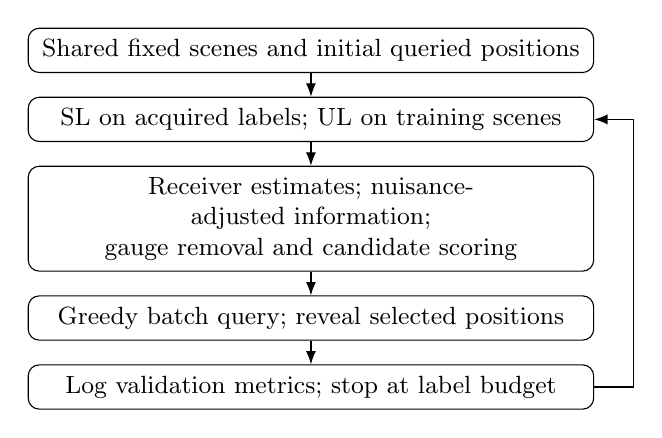
\begin{tikzpicture}[>=Latex,box/.style={draw,rounded corners,align=center,text width=6.9cm,font=\small,inner sep=4pt},node distance=3mm]
\node[box] (pool) {Shared fixed scenes and initial queried positions};
\node[box,below=of pool] (train) {SL on acquired labels; UL on training scenes};
\node[box,below=of train] (score) {Receiver estimates; nuisance-adjusted information;\\gauge removal and candidate scoring};
\node[box,below=of score] (query) {Greedy batch query; reveal selected positions};
\node[box,below=of query] (eval) {Log validation metrics; stop at label budget};
\draw[->] (pool)--(train);
\draw[->] (train)--(score);
\draw[->] (score)--(query);
\draw[->] (query)--(eval);
\draw[->] (eval.east)--++(.5cm,0)|-(train.east);
\end{tikzpicture}
\caption{Implemented acquisition and training cycle. Fresh measurements interrogate fixed scenes. The return path applies while the label budget remains.}\label{fig:workflow}
\end{figure}

\section{Code and Reproducibility}
The original midterm implementation is available in the linked team repository. Updated experiments were performed in a separate local working copy, \texttt{final-report-work/}, preserving the parent reproduction outputs. These local modifications and artifacts must be packaged or committed by the team before claiming that the online repository reproduces the updated tables.

\emph{Full-budget reproduction.} The parent \texttt{results/} folder contains \texttt{SL\_85000.npz}, \texttt{UL\_85000.npz} and \texttt{SSL\_SL\_UL\_1000.npz}; \texttt{methods/show\_results.py} generates the matched-budget plots. The newly executed SL/UL runs used Python 3.12 with PyTorch 2.5.1+cu121 and an RTX 4090. The parent configuration uses seed 42. The original report's seed-10 results are retained as historical comparisons, not pooled with the new seed-42 cohort.

\emph{Corrected acquisition.} \texttt{methods/run\_final\_stage.py} runs the 50-run comparison, noRC controls, summary and transfer ISAC evaluation. Its cohort begins at timestamp \texttt{20261108-142922}; summaries must filter older results. \texttt{methods/run\_followup.py} performs candidate-matrix diagnostics and central-sector evaluation. \texttt{check\_active\_protocol.py} verifies smoke snapshots, shared initialization and the synthetic projection test.

\emph{Hardware study.} \texttt{methods/run\_hardware\_study.py} runs the hardware/coverage factorial. \texttt{lib/hardware.py} uses private hardware seeds; \texttt{check\_hardware.py} verifies reproducibility, array ordering, independent draws and unchanged training randomness. \texttt{ISAC\_RUN\_MODE}, \texttt{ISAC\_COVERAGE}, \texttt{ISAC\_HARDWARE\_SEED} and \texttt{ISAC\_RESULTS\_DIR} select configuration without source edits. The completed cohort is \texttt{hardware\_study\_20261108-160301}. Its manifest records job arguments, exit codes, times and source SHA-256 hashes; an environment snapshot records the interpreter and installed package versions. Every active checkpoint saves true hardware, initial/final queried labels, settings, independent round snapshots and timings. \texttt{summarize\_hardware\_study.py} averages optimizer seeds within hardware before constructing intervals.

\emph{Evaluation and evidence.} \texttt{evaluate\_active\_isac.py} saves per-beam detection, false-alarm, SER and RMSE arrays, test sectors, sample count and seed. It supports transfer and central-sector scenarios. The report embeds new learning curves and tables directly from saved arrays and CSV summaries using \texttt{reports/update\_report.py}; it requires no external image files or bibliography database. Complete clean-environment end-to-end reproduction, independent localization data, unique-label cost accounting and separately calibrated operating points remain outstanding.

\begin{thebibliography}{10}
\providecommand{\url}[1]{#1}
\csname url@samestyle\endcsname
\providecommand{\newblock}{\relax}
\providecommand{\bibinfo}[2]{#2}
\providecommand{\BIBentrySTDinterwordspacing}{\spaceskip=0pt\relax}
\providecommand{\BIBentryALTinterwordstretchfactor}{4}
\providecommand{\BIBentryALTinterwordspacing}{\spaceskip=\fontdimen2\font plus
\BIBentryALTinterwordstretchfactor\fontdimen3\font minus
  \fontdimen4\font\relax}
\providecommand{\BIBforeignlanguage}[2]{{%
\expandafter\ifx\csname l@#1\endcsname\relax
\typeout{** WARNING: IEEEtran.bst: No hyphenation pattern has been}%
\typeout{** loaded for the language `#1'. Using the pattern for}%
\typeout{** the default language instead.}%
\else
\language=\csname l@#1\endcsname
\fi
#2}}
\providecommand{\BIBdecl}{\relax}
\BIBdecl

\bibitem{icc}
J.~M. Mateos-Ramos, C.~H\"ager, M.~F. Keskin, L.~Le~Magoarou, and H.~Wymeersch,
\textquotedblleft Model-driven end-to-end learning for integrated sensing and communication,\textquotedblright{}
in \emph{IEEE ICC}, 2023, pp.~5695--5700, doi: 10.1109/ICC45041.2023.10278889.

\bibitem{multi}
J.~M. Mateos-Ramos, C.~H{\"a}ger, M.~F. Keskin, L.~Le~Magoarou, and
  H.~Wymeersch, ``Model-based end-to-end learning for multi-target integrated
  sensing and communication under hardware impairments,'' \emph{IEEE
  Transactions on Wireless Communications}, vol.~24, no.~3, pp. 2574--2589,
  2025.

\bibitem{ssl}
J.~M. Mateos-Ramos, B.~Chatelier, C.~H{\"a}ger, M.~F. Keskin, L.~Le~Magoarou,
  and H.~Wymeersch, ``Semi-supervised end-to-end learning for integrated
  sensing and communications,'' in \emph{IEEE International Conference on
  Machine Learning for Communication and Networking (ICMLCN)}, 2024, pp.
  132--138.

\bibitem{mbdl}
N.~Shlezinger, J.~Whang, Y.~C. Eldar, and A.~G. Dimakis, \textquotedblleft Model-based deep learning,\textquotedblright{} \emph{Proceedings of the IEEE}, vol.~111, no.~5, pp.~465--499, 2023, doi: 10.1109/JPROC.2023.3247480.

\bibitem{gain}
J.~M. Mateos-Ramos, C.~H{\"a}ger, M.~F. Keskin, L.~Le~Magoarou, and H.~Wymeersch, ``Unsupervised learning for gain-phase impairment calibration in {ISAC}
  systems,'' in \emph{IEEE International Conference on Acoustics, Speech and
  Signal Processing (ICASSP)}, 2025.

\bibitem{music}
B.~Chatelier, J.~M. Mateos-Ramos, V.~Corlay, C.~H{\"a}ger, M.~Crussi{\`e}re,
  H.~Wymeersch, and L.~Le~Magoarou, ``Physically parameterized differentiable
  {MUSIC} for {DoA} estimation with uncalibrated arrays,'' in \emph{IEEE
  International Conference on Communications (ICC)}, 2025, arXiv:2411.15144.

\bibitem{multiul}
J.~M. Mateos-Ramos, B.~Chatelier, L.~Le~Magoarou, N.~Shlezinger, H.~Wymeersch,
  and C.~H{\"a}ger, ``Unsupervised end-to-end array calibration for
  multi-target integrated sensing and communication,'' arXiv preprint
  arXiv:2604.00806, 2026.

\bibitem{weiss}
A.~J. Weiss and B.~Friedlander, \textquotedblleft Array shape calibration using sources in unknown locations---a maximum likelihood approach,\textquotedblright{}
\emph{IEEE Trans. Acoust., Speech, Signal Process.}, vol.~37, no.~12, pp.~1958--1966, 1989, doi: 10.1109/29.45542.

\bibitem{cohn}
D.~A. Cohn, Z.~Ghahramani, and M.~I. Jordan, \textquotedblleft Active learning with statistical models,\textquotedblright{} \emph{Journal of Artificial Intelligence Research}, vol.~4, pp.~129--145, 1996, doi: 10.1613/jair.295.

\bibitem{coreset}
O.~Sener and S.~Savarese, ``Active learning for convolutional neural networks:
  A core-set approach,'' in \emph{International Conference on Learning
  Representations (ICLR)}, 2018, arXiv:1708.00489.

\bibitem{badge}
J.~T. Ash, C.~Zhang, A.~Krishnamurthy, J.~Langford, and A.~Agarwal, ``Deep
  batch active learning by diverse, uncertain gradient lower bounds,'' in
  \emph{International Conference on Learning Representations (ICLR)}, 2020,
  arXiv:1906.03671.

\bibitem{bait}
J.~T. Ash, S.~Goel, A.~Krishnamurthy, and S.~Kakade, ``Gone fishing: Neural
  active learning with fisher embeddings,'' in \emph{Advances in Neural
  Information Processing Systems (NeurIPS)}, 2021, arXiv:2106.09675.

\end{thebibliography}
\end{document}


